\documentclass[ignoreonframetext,unicode]{beamer}

\usepackage[utf8]{inputenc}
\usepackage[T1]{fontenc}
\usepackage[english,russian]{babel}
\usepackage{amsmath}
\usepackage{amsfonts}
\usepackage{amssymb}
\usepackage{graphicx,pgf}
\usepackage{multimedia}

\usetheme{Warsaw}

\useinnertheme{circles}   %внутренняя тема
%\useoutertheme{smoothbars}   %внешняя тема
\usecolortheme{seahorse}     %цветовая схема
%\usefonttheme{serif}    %шрифты
%\defbeamertemplate*{footline}{shadow theme}
%\setbeameroption{hide notes}

\graphicspath{{./style/}{./figures/}}

%номера слайдов
\newcommand*\oldmacro{}%
\let\oldmacro\insertshorttitle%
\renewcommand*\insertshorttitle{%
	\oldmacro\hfill%
	\insertframenumber\,/\,\inserttotalframenumber}
\RequirePackage{caption}
\DeclareCaptionLabelSeparator{defffis}{ }
\captionsetup{justification=centering,labelsep=defffis}

%\title{Курсовая работа}
%\subtitle{Численные схемы для аппроксимации неограниченных решений при моделировании обтекания профиля крыла в вихревых методах}
\title[Решение уравнения Рейнольдса]{Решение уравнения Рейнольдса в рамках теории газовой смазки методом конечных элементов}
\author[Пиневич В.\,Г.]{Докладчик: Пиневич В.\,Г.\and\\[0.5mm] Научный руководитель: Селиванов А.\,В.}

\institute[каф. Прикладная математика ФН-2]{группа ФН2-71Б}
\date{\today}
\titlegraphic{
\includegraphics[width=2cm]{logo.png}}
%\renewcommand{\vec}[1]{\text{\mathversion{bold}${#1}$}}


\begin{document}
	
	\begin{frame}[plain]
		\maketitle
		%\insertshortinstitute{Группа ФН2-41Б}
	\end{frame}

	\begin{frame}{Постановка задачи}
		\vspace*{-4mm}
		\begin{columns}
			\column{\textwidth}`
			\begin{block}{Уравнение Рейнольдса}
			 \[
				\frac{\partial}{\partial x} \left(h^3 \frac{\partial p}{\partial x} \right) + \frac{\partial}{\partial z} \left(h^3 \frac{\partial p}{\partial z} \right) = 6 \mu U \frac{\partial h}{\partial x}
			 \]
			\end{block}

\vspace*{-2mm}
		\begin{columns}
			\column{0.5\textwidth}
			\begin{block}{Граничные условия}
				$U$ --- скорость в направлении $x$,\\ 
				$p_{\text{в}}$ --- повышенное давление,\\ 
				$p_{\text{н}}$ --- пониженное давление
			\end{block}
		
			\column{0.5\textwidth}
			\begin{block}{Описание величин}
			$h = h(x)$ --- толщина слоя, \\
			$p = p(x, z)$ --- давление, \\
			$\mu$ --- коэффициент вязкости
			\end{block}
		\end{columns}

		\end{columns}
		
		\begin{figure}[!htbp]
			\centering
			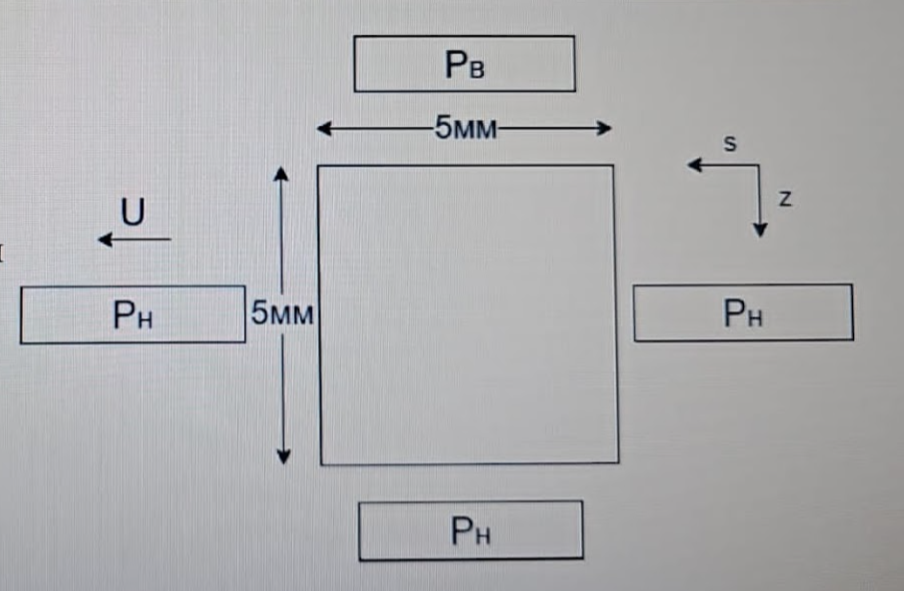
\includegraphics[width=0.4\textwidth]{taskGU}%
			\caption{Cхема области решения задачи}
			\vspace*{-2mm}
			\label{ser_graph}
		\end{figure}
		
	\end{frame}

\begin{frame}{Вывод уравнения Рейнольдса}

\begin{columns}
	\column{0.4\textwidth}
	\begin{block}{Проекции скорости}
		$u$, $\nu$, $\omega$ -- проекции скорости скорости на осях $x$, $y$, $z$ соответственно
	\end{block}
	
	\column{0.6\textwidth}
	\begin{block}{Условие несжимаемости жидкости}	
		\[
		\frac{\partial u}{\partial x} + \frac{\partial \nu}{\partial y} + \frac{\partial \omega}{\partial z} = 0
		\]
	\end{block}
\end{columns}

\begin{columns}
	\column{0.5\textwidth}
\begin{block}{Силы трения в точке}	
	\[
	\begin{cases}
		p_{yz} = p_{zy} = \mu \left(\frac{\partial \omega}{\partial y} + \frac{\partial \nu}{\partial z} \right), \\
		p_{zx} = p_{xz} = \mu \left( \frac{\partial \omega}{\partial x} +  \frac{\partial u}{\partial z} \right), \\
		p_{xy} = p_{yx} = \mu \left(  \frac{\partial u}{\partial y} + \frac{\partial \nu}{\partial x} \right)
	\end{cases}
	\]
\end{block}

\column{0.5\textwidth}
\begin{block}{Давление в
		точке}
	\[
	\begin{cases}
		\frac{\partial p}{\partial x} = \mu \left( \frac{\partial^2 u}{\partial x^2} + \frac{\partial^2 u}{\partial y^2} + \frac{\partial^2 u}{\partial z^2} \right), \\
		\frac{\partial p}{\partial y} = \mu \left( \frac{\partial^2 \nu}{\partial x^2} + \frac{\partial^2 \nu}{\partial y^2} + \frac{\partial^2 \nu}{\partial z^2} \right), \\
		\frac{\partial p}{\partial z} = \mu \left( \frac{\partial^2 \omega}{\partial x^2} + \frac{\partial^2 \omega}{\partial y^2} + \frac{\partial^2 \omega}{\partial z^2} \right)
	\end{cases}
	\]
\end{block}
\end{columns}
	
\end{frame}	

\begin{frame}{}

Изменения скоростей $u$ и $\omega$ со при заданном значении $y$ для всех изменений $ x $ и $z$ могут рассматриваться как чрезмерно малые, поэтому примем
\[
\frac{\partial^2 u}{\partial x^2} = 0, 
\frac{\partial^2 u}{\partial z^2} = 0, 
\frac{\partial^2 \omega}{\partial x^2} = 0, 
\frac{\partial^2 \omega}{\partial z^2} = 0
\]

\begin{columns}

\column{0.5\textwidth}
\begin{block}{}
\[
	\label{secondinitialeq}
	\begin{cases}
		\frac{\partial p }{\partial x} = \mu \frac{\partial^2 u}{\partial y^2}, \\
		\frac{\partial p }{\partial y} = 0, \\
		\frac{\partial p }{\partial z} = \mu \frac{\partial^2 \omega}{\partial y^2}
	\end{cases}
\]
\end{block}

\column{0.5\textwidth}
\begin{block}{}
\[
	\label{secinitialeq}
	\begin{cases}
		p_{yz} = p_{xy} = \mu \frac{\partial \omega}{\partial y}, \\
		p_{zx} = p_{xz} = 0, \\
		p_{xy} = p_{yx} = \mu \frac{\partial u}{\partial y}
	\end{cases}
\]
\end{block}
\end{columns}

\begin{block}{}
\[
	\frac{\partial u}{\partial x} + \frac{\partial \nu}{\partial y} + \frac{\partial \omega}{\partial z} = 0
\]
\end{block}

\end{frame}	

\begin{frame}{}
	
	\begin{columns}
		\column{0.5\textwidth}
		\begin{block}{Для $y = 0$}
			\[
			u = U_0, \nu = 0, \omega = 0
			\]
		\end{block}
	
		\column{0.5\textwidth}
		\begin{block}{Для $y = h$}
		\[
		u = U_1, \nu = U_1 - U_1 \frac{\partial  h}{\partial h}, \omega = 0
		\]
		\end{block}
	\end{columns}


	\begin{block}{}
		\[
		\begin{cases}
			u = \frac{1}{2 \mu} \frac{\partial p}{\partial x} \left( y - h \right) y + U_0 \frac{h - y}{h} + U_1 \frac{y}{h},\\
			\omega = \frac{1}{2 \mu} \frac{\partial p}{\partial z} (y - h) y
		\end{cases}
		\]
	\end{block}
	

	\begin{block}{}
		\[
		\begin{cases}
			p_{yz} = p_{zy} = \frac{1}{2} \frac{\partial p}{\partial z} \left( 2y - h \right), \\
			p_{xy} = p_{yz} = \frac{1}{2} \frac{\partial p}{\partial x} \left( 2y - h \right) + \mu \frac{U_1 - U_0}{h}
		\end{cases}
		\]
	\end{block}


\end{frame}	

\begin{frame}{}
	
	\begin{block}{}
		\[
		\frac{\partial \nu}{\partial y} = - \frac{1}{2 \mu} \frac{\partial}{\partial x} \left( \frac{\partial p}{\partial x} (y - x) y \right) +
		\]
		\[
		+ \frac{\partial}{\partial z} \left( \frac{\partial p}{\partial z} (y - h) h \right) - \frac{\partial}{\partial x} \left( U_0 \frac{h - y}{h} + U_1 \frac{y}{h} \right)
		\]
	\end{block}

Интегрируем это уравнение в пределах от $y = 0$ до $y = h$.
\begin{block}{}
	\[
	\frac{\partial}{\partial x} \left( h^3 \frac{\partial p}{\partial x} \right) + \frac{\partial}{\partial z} \left( h^3 \frac{\partial p}{\partial z} \right) = 6 \mu \left( (U_0 - U_1) \frac{\partial h}{\partial x} \right) + 2 V_1
	\]
\end{block}
$2 V_1$ используется для учёта движений одной из стенок зазора, меняющих значение функции. Если пренебречь этим, и обозначить $U_0 - U_1$ как $U$, то получим искомое уравнение
	
\end{frame}

\begin{frame}{Решение уравнения Рейнольдса с помощью слабой формы Галеркина}
	
\begin{columns}
		
		\column{0.5\textwidth}
	\begin{block}{Функции формы}
		\[
			\begin{cases}
				N_1 = 1 - \frac{x}{l} - \frac{z}{h} + \frac{x  z}{l  h}, \\
				N_2 = \frac{x}{l} - \frac{x  z}{l  h}, \\
				N_3 = \frac{x  z}{l h}, \\
				N_4 = \frac{z}{h} - \frac{x  z}{l  h} \\
			\end{cases}
			\label{form-func}
		\]
		\end{block}
	
	\column{0.5\textwidth}
	\begin{block}{Входные данные}
	\[
		\begin{cases}
			h = 0.0001 \text{ м}, \\
			verticalLength = 0.005 \text{ м}, \\
			horizontalLength = 0.005 \text{ м}, \\
			\mu = 8.90 * 10^{-4} \text{ Па}*\text{с}, \\
			U = 10 \text{ м/c}, \\
			p_{\text{н}} = 100 \text{ кПа}, \\
			p_{\text{в}} = 150 \text{ кПа} \\
		\end{cases}	
	\]
\end{block}
\end{columns}

\begin{block}{Аппроксимирующая функция}
	\[
	\phi = c_0 N_1 + c_1 N_2 + c_2 N_3 + c_3 N_4
	\]
\end{block}
	
\end{frame}

\begin{frame}{Решение на сетке 10 на 10}
	
	\begin{columns}
		
		\column{0.5\textwidth}
		\begin{figure}[!htbp]
			\center{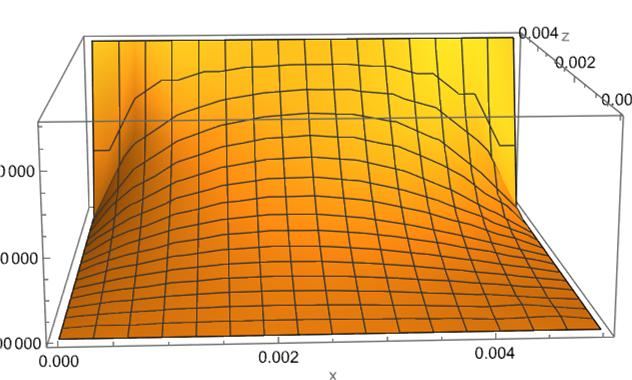
\includegraphics[width=\textwidth, height=0.5\textwidth]{10x10mesh.jpg}}
			\caption{График решения уравнения Рейнольдса для h = 0.0001 м на сетке 10 на 10 элементов}
			\label{10x10mesh}
		\end{figure}
		
		\column{0.5\textwidth}
		\begin{figure}[!htbp]
			\center{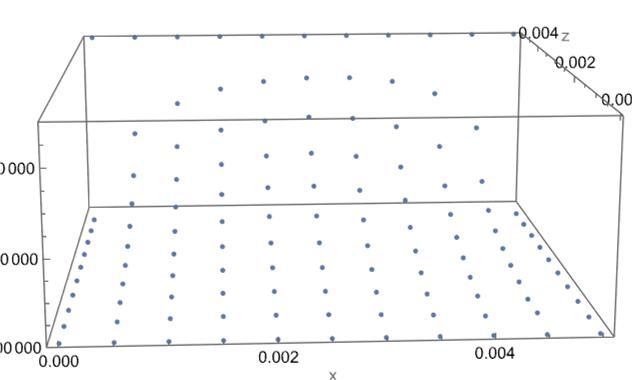
\includegraphics[width=\textwidth, height=0.5\textwidth]{10x10points.jpg}}
			\caption{График значений узлов решения уравнения Рейнольдса для h = 0.0001 м на сетке 10 на 10 элементов}
			\label{10x10points}
		\end{figure}
		
	\end{columns}
	
\end{frame}

\begin{frame}{Решение на сетке 20 на 20}
	
	\begin{columns}
		
		\column{0.5\textwidth}
		\begin{figure}[!htbp]
			\center{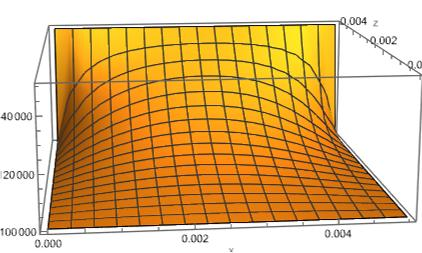
\includegraphics[width=\textwidth, height=0.5\textwidth]{20x20mesh.jpg}}
			\caption{График решения уравнения Рейнольдса для h = 0.0001 м на сетке 20 на 20 элементов}
			\label{5x5mesh}
		\end{figure}
		
		\column{0.5\textwidth}
		\begin{figure}[!htbp]
			\center{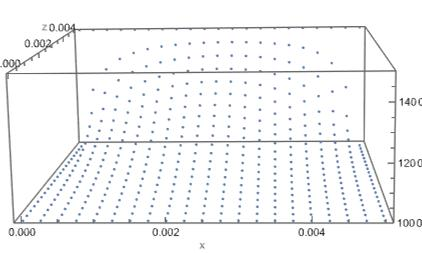
\includegraphics[width=\textwidth, height=0.5\textwidth]{20x20points.jpg}}
			\caption{График значений узлов решения уравнения Рейнольдса для h = 0.0001 м на сетке 20 на 20 элементов}
			\label{20x20points}
		\end{figure}
		
	\end{columns}
	
\end{frame}

\begin{frame}{Сравнение решения с Wolfram Mathematica}
	\vspace*{-4mm}
	\begin{figure}[!htbp]
		\center{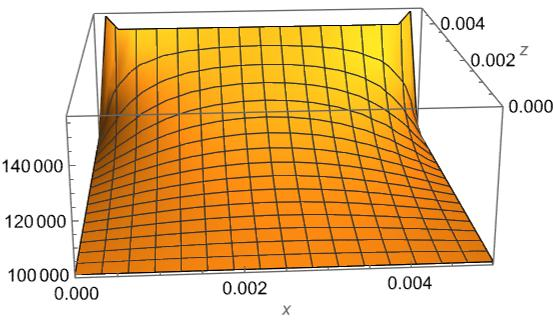
\includegraphics[width=\textwidth, height=0.4\textwidth]{exactSolutionConst.jpg}}
		\caption{График решения уравнения Рейнольдса для h = 0.0001 м полученный с помощью Wolfram Mathematica}
		\label{exactSolutionConst}
	\end{figure}

\begin{table}[!htbp]
	\begin{tabular}{|l|l|l|}
		\hline
		\multicolumn{1}{|c|}{Размерность сетки} & \multicolumn{1}{c|}{Разность, Па} & Погрешность, \% \\ \hline
		5 на 5                                  & 4612                              & 4.51            \\ \hline
		10 на 10                                & 1538                              & 1.38            \\ \hline
		20 на 20                                & 1290                              & 1.02            \\ \hline
	\end{tabular}
\end{table}
\end{frame}

\begin{frame}{Заключение}
	В работе представлен вывод уравнения Рейнольдса для установившегося течения в газовом смазочном слое и методика реmшения уравнения Рейнольдса с помощью метода конечных элементов. В ходе работы получены следующие результаты:
	\begin{block}{}
	\begin{enumerate}	
		\item Создана программная реализация метода конечного элемента для решение уравнения Рейнольдса
		\item Полученные значения решения уравнения Рейнольдса были сравнены с результатами решения, полученного с помощью функции NDSolve в Wolfram Mathematica
		\item В результате сравнения для сетки 5 на 5 погрешность равна 4.51 \%, а для сетки 20 на 20 -- 1.02 \%.
	\end{enumerate}
	\end{block}	
\end{frame}	
\end{document} 